    \chapter*{chapitre 2}
    
    \markboth{Chapitre 2 }{ Analyse et spécification des besoins} %pour afficher l'entete
    \addcontentsline{toc}{chapter}{2  Analyse et spécification des besoins}
    \textbf{\Huge Analyse et spécification des besoins}
    
    \setcounter{chapter}{2}
    \setcounter{section}{0}
    
    
    \section{Introduction}
    
    Après avoir présenté, au chapitre précédent, le contexte général du projet ainsi que la solution retenue, ce chapitre a pour objectif de spécifier précisément les besoins auxquels la plateforme doit répondre, puis de fournir une vue d'ensemble de l'analyse globale du système et de son pilotage. Nous identifions dans un premier temps les différents acteurs qui interagissent avec le système, puis nous détaillons les besoins fonctionnels et non fonctionnels, ainsi que le diagramme de cas d'utilisation général. Nous présentons ensuite l'analyse globale de la plateforme (diagramme de classes d'analyse et architecture logique/physique), le pilotage du projet avec la méthode Scrum, avant de clore le chapitre par la description de l'environnement de travail utilisé pour la réalisation du projet.
    
    
    \section{Modélisation du contexte}
    
    \subsection{Identification des acteurs}
    
    L'analyse de la documentation fonctionnelle de la plateforme permet d'identifier trois acteurs principaux, correspondant aux rôles gérés par le module de sécurité (Keycloak et couche d'autorisation applicative) :
    
    \begin{itemize}
        \item \textbf{Administrateur de la plateforme (ADMIN)} : représente l'équipe opérationnelle de NextStep IT en charge de l'exploitation de la plateforme. Il supervise l'ensemble des clients (tenants), le cluster Kubernetes, la facturation globale, les quotas, et intervient via la console d'administration dédiée.
    
        \item \textbf{Administrateur de compte client (CLIENT\_ADMIN)} : représente le responsable, côté client, d'un compte locataire de la plateforme. Il gère son équipe (invitation de membres), configure et déploie ses applications, consulte sa facturation, et dispose de la totalité des permissions sur les ressources de son compte.
    
        \item \textbf{Membre d'équipe (MEMBER)} : utilisateur rattaché à un compte client, disposant d'un sous-ensemble de permissions accordées explicitement par le CLIENT\_ADMIN (par exemple : déployer une application, consulter les journaux, consulter la supervision, gérer Kafka ou l'Eventing), sans nécessairement disposer de l'ensemble des droits du compte.
    \end{itemize}
    
    
    
    \subsection{Spécification des besoins}
    
    \subsubsection{Besoins fonctionnels}
    \label{sec:besoins-fonctionnels}
    
    Les besoins fonctionnels sont organisés ci-dessous selon les grands blocs fonctionnels et techniques de la plateforme, qui seront repris sous forme d'epics dans le Product Backlog présenté en section~\ref{sec:scrum}.
    
    \paragraph{Infrastructure Cloud Native.} Le système doit reposer sur un cluster Kubernetes offrant l'isolation des ressources par tenant (espace de noms dédié par client), un adressage réseau maîtrisé (répartiteur de charge, passerelle d'entrée) et des règles d'isolation réseau entre locataires.
    
    \paragraph{Plateforme Serverless.} Le système doit permettre à un client de déployer une application à partir d'une image Docker existante, de définir le port d'écoute, les ressources allouées (CPU, mémoire), ainsi que les bornes de mise à l'échelle (nombre minimum et maximum de réplicas, y compris la possibilité de descendre à zéro instance en l'absence de trafic). Le système doit assurer le suivi de l'état de déploiement de l'application en temps réel, permettre sa mise à jour, sa suppression logique (conservation de l'historique de facturation), la consultation de son historique de révisions et le retour (\textit{rollback}) vers une révision antérieure.
    
    \paragraph{Messaging Kafka.} Le système doit permettre à un client de créer et de gérer des sujets (\textit{topics}) Kafka associés à son compte, en vue d'un usage applicatif de messagerie asynchrone.
    
    \paragraph{Backend Spring Boot.} Le système doit exposer une API REST sécurisée couvrant l'ensemble des fonctionnalités métier (gestion des utilisateurs et des permissions, gestion des applications, facturation, clés d'API, journaux de déploiement), et orchestrer les ressources Kubernetes/Knative/Strimzi correspondantes de manière transparente pour l'utilisateur.
    
    \paragraph{Knative Eventing.} Le système doit permettre de relier un sujet Kafka à une application déployée, de sorte qu'un message publié sur ce sujet puisse déclencher automatiquement le réveil (remise à l'échelle depuis zéro instance) et l'invocation de l'application concernée.
    
    \paragraph{Frontend React.} Le système doit fournir un portail web pour les clients (déploiement et supervision de leurs applications, consultation de la facturation, gestion d'équipe) ainsi qu'une console d'administration séparée pour l'équipe exploitant la plateforme (supervision du cluster, gestion des comptes clients, facturation globale, journal d'audit).
    
    \paragraph{Monitoring \& Observabilité.} Le système doit fournir aux clients une visibilité sur l'état et les journaux de leurs applications (journaux de déploiement, journaux applicatifs, métriques), et à l'équipe d'exploitation une visibilité sur l'état global du cluster (nœuds, charge, alertes actives), ainsi qu'un mécanisme de détection automatique des redémarrages en boucle des applications.
    
    \paragraph{CI/CD.} Le système doit permettre la construction, la publication et le déploiement automatisés des composants de la plateforme elle-même (backend, portail client, console d'administration) à chaque évolution du code source.
    
    \subsubsection{Besoins non fonctionnels}
    
    \begin{itemize}
        \item \textbf{Isolation multi-tenant} : les ressources et les données d'un client ne doivent en aucun cas être accessibles par un autre client. Cette isolation doit être assurée à la fois au niveau applicatif (contrôle d'accès basé sur le propriétaire effectif de la ressource) et au niveau réseau (règles d'isolation entre espaces de noms Kubernetes).
        \item \textbf{Élasticité et efficience des ressources} : la plateforme doit permettre à une application de ne consommer aucune ressource de calcul lorsqu'elle est inactive (mise à l'échelle à zéro), et de monter en charge automatiquement en fonction du trafic reçu.
        \item \textbf{Facturation à l'usage} : le coût facturé à un client doit refléter la consommation réelle de ses applications (temps d'activité, ressources allouées), et non un forfait fixe indépendant de l'usage.
        \item \textbf{Sécurité} : l'authentification des utilisateurs doit reposer sur un fournisseur d'identité centralisé, les autorisations doivent être vérifiées à chaque accès à une ressource, et les échanges sensibles (jetons d'authentification) ne doivent pas être exposés inutilement (par exemple dans les journaux ou les paramètres d'URL).
        \item \textbf{Disponibilité} : les composants de la plateforme elle-même (backend, portails, briques d'infrastructure) doivent pouvoir être redéployés sans interruption prolongée de service, et le système doit permettre de détecter automatiquement une dégradation (redémarrages en boucle, alertes).
        \item \textbf{Observabilité} : l'état du système, à tous les niveaux (infrastructure, plateforme, applications clientes), doit pouvoir être supervisé au travers d'outils de métriques et de tableaux de bord.
        \item \textbf{Automatisation} : la construction et le déploiement des composants de la plateforme doivent être automatisés afin de réduire les erreurs manuelles et le délai de mise en production d'une évolution.
    \end{itemize}
    
    \subsection{Diagramme de cas d'utilisation général}
    
    Les diagrammes de cas d'utilisation globaux des figures~\ref{fig:uc-global} et~\ref{fig:uc-global-admin} synthétisent les interactions entre les trois acteurs identifiés et les grandes fonctionnalités de la plateforme, respectivement côté client (CLIENT\_ADMIN/MEMBER) et côté administration (ADMIN). Les cas d'utilisation spécifiques à chaque fonctionnalité (par exemple : « Déployer une application », « Créer un sujet Kafka », « Configurer un déclencheur d'événement ») sont détaillés, avec leur description textuelle et, le cas échéant, leur diagramme de séquence, dans le chapitre de réalisation correspondant au Sprint qui les a implémentés.
    
    \begin{flushleft}
    
    \begin{figure}[H]
     \centering
        
\includegraphics[width=9cm]{image/usescasememeberadmin.png}
        \caption{Diagramme de cas d'utilisation global de la plateforme — CLIENT\_ADMIN et MEMBER}
        \label{fig:uc-global}
    \end{figure}
    
    \begin{figure}[H]
     \centering
        
\includegraphics[width=9cm]{image/diagrameadmin.png}
        \caption{Diagramme de cas d'utilisation global de la plateforme — ADMIN}
        \label{fig:uc-global-admin}
    \end{figure}
    
    \end{flushleft}
    
    Le tableau~\ref{tab:uc-global} récapitule les principaux cas d'utilisation du système, l'acteur concerné, ainsi que le sprint de réalisation correspondant, permettant au lecteur de faire le lien avec les chapitres de réalisation.
    
    \begin{table}[!ht]
    \begin{center}
         \begin{tabular}{|l{6cm}|l{4cm}|l{2cm}|}
         \hline
         \textbf{Cas d'utilisation} & \textbf{Acteur(s)} & \textbf{Sprint} \\
         \hline
         Se connecter à la plateforme & CLIENT\_ADMIN, MEMBER, ADMIN & Sprint 4 \\
         \hline
         Gérer les membres de l'équipe & CLIENT\_ADMIN & Sprint 4 \\
         \hline
         Déployer une application & CLIENT\_ADMIN, MEMBER & Sprint 5 \\
         \hline
         Mettre à jour / supprimer une application & CLIENT\_ADMIN, MEMBER & Sprint 5 \\
         \hline
         Consulter l'historique de révisions et effectuer un rollback & CLIENT\_ADMIN, MEMBER & Sprint 5 \\
         \hline
         Créer et gérer un sujet Kafka & CLIENT\_ADMIN, MEMBER & Sprint 6 \\
         \hline
         Configurer un déclencheur d'événement (Trigger/KafkaSource) & CLIENT\_ADMIN, MEMBER & Sprint 6 \\
         \hline
         Consulter les journaux et les métriques d'une application & CLIENT\_ADMIN, MEMBER & Sprint 7 \\
         \hline
         Consulter sa facturation & CLIENT\_ADMIN & Sprint 7 \\
         \hline
         Superviser le cluster (nœuds, alertes, tenants) & ADMIN & Sprint 7 \\
         \hline
         Gérer les comptes clients et les quotas & ADMIN & Sprint 7 \\
         \hline
         Générer une clé d'API pour un pipeline CI/CD & CLIENT\_ADMIN & Sprint 5 \\
         \hline
         \end{tabular}
         \caption{Principaux cas d'utilisation de la plateforme et sprint de réalisation associé}
         \label{tab:uc-global}
         \end{center}
         \end{table}
    
    
    \section{Analyse Globale}
    
    Cette section donne une vue d'ensemble cohérente de l'architecture logique et physique du système, des composants qui le constituent et de leurs interactions, ainsi que des processus métier les plus structurants — indépendamment du découpage en sprints qui structurera les chapitres suivants. Les diagrammes UML propres à une fonctionnalité particulière (par exemple le diagramme de séquence détaillé de la création d'un déclencheur Kafka) seront présentés dans le chapitre de réalisation correspondant, en cohérence avec la vue d'ensemble donnée ici.
    
    \subsection{Diagramme de classes d'analyse}
    
    Le diagramme de classes de la figure~\ref{fig:classes-global} présente les entités métier centrales du système et leurs relations : \texttt{User} (avec son rôle \texttt{UserRole} — ADMIN, CLIENT\_ADMIN, MEMBER — et ses permissions individuelles), \texttt{App} (l'application déployée par un client, avec son statut et ses paramètres de mise à l'échelle), \texttt{DeploymentLog} (historique des événements de cycle de vie d'une application), \texttt{BillingSnapshot} et \texttt{AppInvoice} (facturation), ainsi que les entités liées aux clés d'API. La classe \texttt{User} est reliée à \texttt{App} par une relation de propriété, résolue à l'exécution par le service \texttt{UserContextService} qui rattache systématiquement les ressources d'un \texttt{MEMBER} à son \texttt{CLIENT\_ADMIN} (modèle de délégation de propriété).
    
    \begin{figure}[h!]
     \centering
        
\includegraphics[width=13.5cm]{image/class1.png}
        \caption{Diagramme de classe général}
        \label{fig:classes-global}
    \end{figure}
    
    \subsection{Architecture globale}
    
    \subsubsection{Architecture logique de la plateforme}
    
    L'architecture logique de la plateforme est organisée en quatre couches, représentées à la figure~\ref{fig:archi-logique} :
    
    \begin{itemize}
        \item \textbf{Couche présentation} : deux applications monopage (SPA) développées en React — le \textit{portail client} (déploiement et supervision des applications, facturation, gestion d'équipe) et la \textit{console d'administration} (supervision du cluster, gestion des comptes clients, facturation globale, audit) — toutes deux servies statiquement via Nginx.
        \item \textbf{Couche service} : une API REST unique développée en Spring Boot (module \texttt{backend-api}), organisée par domaine métier (applications, facturation, utilisateurs, Kafka, Eventing, clés d'API, journaux, administration), qui centralise l'ensemble de la logique métier et constitue le point d'entrée unique vers le cluster Kubernetes.
        \item \textbf{Couche orchestration} : le client Kubernetes Java \textbf{Fabric8}, utilisé par la couche service pour créer, lire, modifier et surveiller les ressources Kubernetes natives ainsi que les ressources personnalisées (CRD) de Knative Serving, Knative Eventing et Strimzi.
        \item \textbf{Couche infrastructure} : le cluster Kubernetes et les opérateurs qui y sont déployés (Knative Serving, Knative Eventing, Strimzi/Kafka), ainsi que les briques transverses — Keycloak (identité), PostgreSQL (persistance), Prometheus/Grafana (supervision), Jenkins/Kaniko (intégration et déploiement continus).
    \end{itemize}
    
    \begin{figure}[h!]
     \centering
        
\includegraphics[width=13.5cm]{image/logique.png}
        \caption{Architecture logique de la plateforme}
        \label{fig:archi-logique}
    \end{figure}
    
    Un principe de conception central de cette architecture est que \textbf{le backend Spring Boot est l'unique point d'entrée autorisé vers le cluster} : ni les portails React, ni les clients externes (pipelines CI/CD via clé d'API) n'interagissent directement avec l'API Kubernetes. Ce choix garantit que toute action sur le cluster passe par les contrôles d'authentification, d'autorisation et d'appartenance (isolation multi-tenant) implémentés dans la couche service.
    
    \subsubsection{Architecture physique de la plateforme}
    
    La figure~\ref{fig:archi-physique} présente l'architecture physique (diagramme de déploiement) de la plateforme telle qu'exploitée sur le cluster Kubernetes décrit en section~\ref{sec:env-materiel}.
    
    \begin{figure}[h!]
     \centering
        
\includegraphics[width=13.5cm]{image/physiquearchitecture.png}
        \caption{Diagramme de déploiement de la plateforme}
        \label{fig:archi-physique}
    \end{figure}
    
    Les éléments principaux de ce déploiement sont :
    
    \begin{itemize}
        \item Chaque \textbf{tenant} (client) dispose de son propre espace de noms (\textit{namespace}) Kubernetes, isolé des autres tenants par une ressource \texttt{NetworkPolicy} créée automatiquement à la première utilisation.
        \item Les applications des clients sont déployées comme des ressources \texttt{Service} de Knative Serving à l'intérieur de leur espace de noms respectif ; chaque service Knative peut être instancié en zéro, une ou plusieurs révisions actives (\textit{Revision}) selon la charge.
        \item Le backend, les deux portails React, Keycloak et PostgreSQL sont déployés dans un espace de noms dédié à la plateforme (\texttt{platform}), distinct des espaces de noms des tenants.
        \item Un cluster Kafka, opéré par Strimzi, héberge les sujets (\textit{topics}) créés par les clients ; Knative Eventing s'interface avec ce cluster via les ressources \texttt{KafkaSource}, \texttt{Broker} et \texttt{Trigger}.
        \item L'accès externe au cluster est assuré par MetalLB (attribution d'adresses IP de type \textit{LoadBalancer}) et par la passerelle Kourier pour le trafic à destination des services Knative.
    \end{itemize}
    
    \subsubsection{Diagramme de composants}
    
    Le diagramme de composants de la figure~\ref{fig:archi-composants} détaille les principaux modules internes du backend Spring Boot et leurs dépendances, organisés par domaine métier (\textit{package-by-feature}) : gestion des applications (\texttt{app}), facturation (\texttt{billing}), utilisateurs et permissions (\texttt{user}), sécurité (\texttt{security}), clés d'API (\texttt{apikey}), Kafka (\texttt{kafka}), Eventing (\texttt{eventing}), administration (\texttt{admin}) et journaux (\texttt{logs}). Chacun de ces modules s'appuie sur un client Fabric8 partagé pour ses interactions avec le cluster Kubernetes, et sur une base PostgreSQL commune pour la persistance de ses entités.
    
    \begin{figure}[h!]
     \centering
        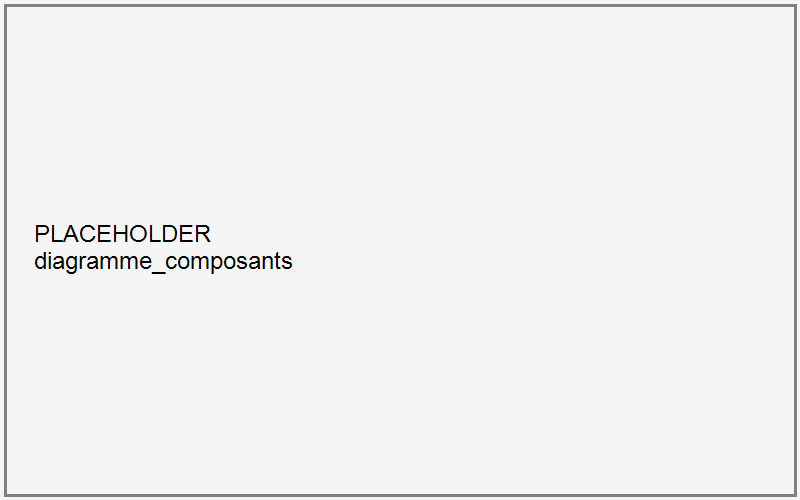
\includegraphics[width=13.5cm]{diagrammes/diagramme_composants.png}
        \caption{Diagramme de composants du backend}
        \label{fig:archi-composants}
    \end{figure}
    
    \subsubsection{Processus métier principaux}
    
    Cette section présente les diagrammes de séquence des processus transverses les plus structurants du système, communs à plusieurs sprints de réalisation. Les diagrammes de séquence propres à une fonctionnalité précise et localisée à un seul sprint seront, quant à eux, présentés directement dans le chapitre correspondant.
    
    \paragraph{Processus de déploiement d'une application.} Le processus de déploiement, illustré à la figure~\ref{fig:seq-deploiement}, se déroule selon les étapes suivantes :
    
    \begin{enumerate}
        \item Le client renseigne le formulaire de déploiement (nom, image Docker, port, ressources, bornes de mise à l'échelle) sur le portail.
        \item Le portail envoie une requête \texttt{POST /api/apps} au backend.
        \item Le backend résout l'identité effective de l'appelant (délégation MEMBER $\rightarrow$ CLIENT\_ADMIN), puis génère un nom de service unique compatible DNS.
        \item L'entité \texttt{App} est immédiatement persistée avec le statut \texttt{DEPLOYING}, un \texttt{DeploymentLog} est créé et diffusé en temps réel au portail via un flux d'événements serveur (SSE).
        \item Le backend répond immédiatement au client, \textbf{avant} que le déploiement effectif sur le cluster ne soit terminé.
        \item De manière asynchrone, le backend s'assure de l'existence de l'espace de noms du tenant et de sa \texttt{NetworkPolicy}, puis crée la ressource \texttt{Service} de Knative Serving correspondante.
        \item Knative crée une \texttt{Revision} et une \texttt{Route} ; le pod applicatif démarre (ou reste à zéro instance si le minimum de réplicas est nul).
        \item Un observateur (\textit{watcher}) Fabric8 met à jour le statut de l'application en base de données au fil de l'évolution de l'état réel du cluster, et le portail reflète ce statut en temps réel.
    \end{enumerate}
    
    
    
    \paragraph{Processus événementiel Kafka vers Knative.} Le processus déclenché par la réception d'un message Kafka, illustré à la figure~\ref{fig:seq-eventing}, se déroule selon les étapes suivantes :
    
    \begin{enumerate}
        \item Un producteur publie un message sur un sujet Kafka du cluster Strimzi.
        \item La ressource \texttt{KafkaSource}, associée à ce sujet, consomme le message et l'encapsule au format \textit{CloudEvent}, avant de le transmettre par requête HTTP au \textit{Broker} de Knative Eventing.
        \item Le \textit{Broker} évalue les filtres définis par les ressources \texttt{Trigger} enregistrées et transmet l'événement à l'application abonnée correspondante.
        \item Si l'application cible est à zéro instance, l'\textit{Activator} de Knative intercepte la requête, la met en attente, et déclenche la remise à l'échelle du service.
        \item Une fois l'instance disponible, l'application traite l'événement reçu et retourne une réponse HTTP 200.
        \item En l'absence de nouvelle sollicitation, l'application redescend automatiquement à zéro instance après une période d'inactivité.
    \end{enumerate}
    
    
    
    \section{Pilotage du projet avec SCRUM}
    \label{sec:scrum}
    
    Le cadre agile \textbf{Scrum}, retenu au chapitre précédent pour la conduite de ce projet, structure le développement en itérations courtes et fixes appelées \textit{sprints}, à l'issue desquelles un incrément de produit potentiellement livrable est produit.
    
    \subsection{Backlog du produit}
    
    Le tableau~\ref{tab:backlog} présente le backlog du produit de la plateforme. Les fonctionnalités sont organisées par module — en cohérence directe avec les besoins fonctionnels spécifiés en section~\ref{sec:besoins-fonctionnels} — et décrites sous forme de \textit{User Stories}.
    
    \refstepcounter{table}
    \label{tab:backlog}
    \begin{center}
    \textbf{\tablename~\thetable\ -- Backlog du produit}
    \end{center}
    \addcontentsline{lot}{table}{\protect\numberline{\thetable}Backlog du produit}
    
    {\small
    \renewcommand{\arraystretch}{1.3}
    \setlength{\tabcolsep}{4pt}
    \begin{longtable}{|>{\centering\arraybackslash}m{0.8cm}|>{\centering\arraybackslash}m{2.6cm}|>{\centering\arraybackslash}m{1.1cm}|>{\raggedright\arraybackslash}p{6.1cm}|>{\centering\arraybackslash}m{2.3cm}|}
    \hline
    \rowcolor{Gray}
    \textbf{ID} & \textbf{Module} & \textbf{ID US} & \textbf{User Story} & \textbf{Complexité} \\
    \hline
    \endfirsthead
    
    \hline
    \rowcolor{Gray}
    \textbf{ID} & \textbf{Module} & \textbf{ID US} & \textbf{User Story} & \textbf{Complexité} \\
    \hline
    \endhead
    
    \hline
    \multicolumn{5}{r{12.9cm}}{\textit{Suite à la page suivante}} \\
    \endfoot
    
    \endlastfoot
    
    %=========================================================
    % M1
    %=========================================================
    \multirow{5}{*}{M1} & \multirow{5}{2.6cm}{\centering Authentification \& Sécurité}
     & M1.1 & En tant qu'utilisateur, je souhaite me connecter à la plateforme via Keycloak. & Moyenne \\
    \cline{3-5}
     && M1.2 & En tant qu'utilisateur, je souhaite me déconnecter du système. & Faible \\
    \cline{3-5}
     && M1.3 & En tant qu'utilisateur, je souhaite que mon jeton d'authentification (JWT) soit automatiquement rafraîchi. & Moyenne \\
    \cline{3-5}
     && M1.4 & En tant qu'administrateur, je souhaite définir les rôles et les permissions des utilisateurs. & Élevée \\
    \cline{3-5}
     && M1.5 & En tant qu'utilisateur, je souhaite générer une clé d'API pour piloter mes déploiements depuis un pipeline CI/CD externe. & Moyenne \\
    \hline
    
    %=========================================================
    % M2
    %=========================================================
    \multirow{4}{*}{M2} & \multirow{4}{2.6cm}{\centering Utilisateurs \& équipes}
     & M2.1 & En tant qu'administrateur de compte client, je souhaite inviter un membre dans mon équipe. & Moyenne \\
    \cline{3-5}
     && M2.2 & En tant qu'administrateur de compte client, je souhaite modifier les permissions d'un membre de mon équipe. & Moyenne \\
    \cline{3-5}
     && M2.3 & En tant qu'administrateur de compte client, je souhaite retirer un membre de mon équipe. & Faible \\
    \cline{3-5}
     && M2.4 & En tant qu'administrateur de la plateforme, je souhaite gérer les comptes clients (activation, suspension, quotas). & Élevée \\
    \hline
    
    %=========================================================
    % M3
    %=========================================================
    \multirow{3}{*}{M3} & \multirow{3}{2.6cm}{\centering Infrastructure Cloud Native}
     & M3.1 & En tant que système, je souhaite créer automatiquement un espace de noms (namespace) dédié pour chaque nouveau tenant. & Élevée \\
    \cline{3-5}
     && M3.2 & En tant que système, je souhaite appliquer automatiquement une NetworkPolicy isolant chaque tenant. & Élevée \\
    \cline{3-5}
     && M3.3 & En tant qu'administrateur, je souhaite superviser l'état des nœuds du cluster Kubernetes. & Moyenne \\
    \hline
    
    %=========================================================
    % M4
    %=========================================================
    \multirow{7}{*}{M4} & \multirow{7}{2.6cm}{\centering Gestion des applications}
     & M4.1 & En tant qu'utilisateur, je souhaite déployer une application à partir d'une image Docker. & Élevée \\
    \cline{3-5}
     && M4.2 & En tant qu'utilisateur, je souhaite définir les ressources (CPU, mémoire) et les bornes de mise à l'échelle de mon application. & Moyenne \\
    \cline{3-5}
     && M4.3 & En tant qu'utilisateur, je souhaite mettre à jour la configuration d'une application déjà déployée. & Moyenne \\
    \cline{3-5}
     && M4.4 & En tant qu'utilisateur, je souhaite supprimer une application (suppression logique, conservation de l'historique de facturation). & Moyenne \\
    \cline{3-5}
     && M4.5 & En tant qu'utilisateur, je souhaite consulter l'historique des révisions d'une application. & Moyenne \\
    \cline{3-5}
     && M4.6 & En tant qu'utilisateur, je souhaite effectuer un rollback vers une révision antérieure. & Élevée \\
    \cline{3-5}
     && M4.7 & En tant qu'utilisateur, je souhaite suivre en temps réel le statut de déploiement de mon application. & Élevée \\
    \hline
    
    %=========================================================
    % M5
    %=========================================================
    \multirow{3}{*}{M5} & \multirow{3}{2.6cm}{\centering Messaging Kafka}
     & M5.1 & En tant qu'utilisateur, je souhaite créer un sujet (topic) Kafka pour mon compte. & Moyenne \\
    \cline{3-5}
     && M5.2 & En tant qu'utilisateur, je souhaite consulter la liste des sujets Kafka de mon compte. & Faible \\
    \cline{3-5}
     && M5.3 & En tant qu'utilisateur, je souhaite supprimer un sujet Kafka. & Faible \\
    \hline
    
    %=========================================================
    % M6
    %=========================================================
    \multirow{3}{*}{M6} & \multirow{3}{2.6cm}{\centering Knative Eventing}
     & M6.1 & En tant qu'utilisateur, je souhaite relier un sujet Kafka à une de mes applications déployées. & Élevée \\
    \cline{3-5}
     && M6.2 & En tant qu'utilisateur, je souhaite que mon application soit automatiquement réveillée (scale depuis zéro) à la réception d'un événement. & Élevée \\
    \cline{3-5}
     && M6.3 & En tant qu'utilisateur, je souhaite configurer un déclencheur (Trigger) avec un filtre sur le type d'événement. & Moyenne \\
    \hline
    
    %=========================================================
    % M7
    %=========================================================
    \multirow{3}{*}{M7} & \multirow{3}{2.6cm}{\centering Facturation}
     & M7.1 & En tant qu'utilisateur, je souhaite consulter la facturation de mes applications basée sur leur usage réel. & Élevée \\
    \cline{3-5}
     && M7.2 & En tant qu'administrateur, je souhaite consulter la facturation globale de tous les comptes clients. & Moyenne \\
    \cline{3-5}
     && M7.3 & En tant qu'utilisateur, je souhaite recevoir une alerte lorsque mon budget approche un seuil défini. & Moyenne \\
    \hline
    
    %=========================================================
    % M8
    %=========================================================
    \multirow{4}{*}{M8} & \multirow{4}{2.6cm}{\centering Monitoring \& Observabilité}
     & M8.1 & En tant qu'utilisateur, je souhaite consulter les journaux applicatifs de mon application en temps réel (SSE). & Élevée \\
    \cline{3-5}
     && M8.2 & En tant qu'utilisateur, je souhaite consulter les métriques (CPU, mémoire, requêtes) de mon application. & Moyenne \\
    \cline{3-5}
     && M8.3 & En tant qu'administrateur, je souhaite être alerté automatiquement en cas de redémarrage en boucle (crash loop) d'une application. & Élevée \\
    \cline{3-5}
     && M8.4 & En tant qu'administrateur, je souhaite consulter un tableau de bord Grafana de l'état global du cluster. & Moyenne \\
    \hline
    
    %=========================================================
    % M9
    %=========================================================
    \multirow{2}{*}{M9} & \multirow{2}{2.6cm}{\centering Administration plateforme}
     & M9.1 & En tant qu'administrateur, je souhaite consulter le journal d'audit des actions effectuées sur la plateforme. & Moyenne \\
    \cline{3-5}
     && M9.2 & En tant qu'administrateur, je souhaite gérer les quotas alloués à chaque compte client. & Moyenne \\
    \hline
    
    %=========================================================
    % M10
    %=========================================================
    \multirow{3}{*}{M10} & \multirow{3}{2.6cm}{\centering CI/CD}
     & M10.1 & En tant qu'équipe de développement de la plateforme, je souhaite que chaque évolution du code source déclenche automatiquement la construction d'une image Docker via Kaniko. & Élevée \\
    \cline{3-5}
     && M10.2 & En tant qu'équipe de développement de la plateforme, je souhaite que l'image construite soit automatiquement publiée sur le registre Docker Hub. & Moyenne \\
    \cline{3-5}
     && M10.3 & En tant qu'équipe de développement de la plateforme, je souhaite que la nouvelle version soit automatiquement déployée sur le cluster après publication. & Élevée \\
    \hline
    \end{longtable}
    }
    
    \subsection{Planification des Sprints}
    
    La planification cible retenue pour la conduite du projet, définissant l'ordre logique de construction des différentes briques de la plateforme, est présentée dans le tableau~\ref{tab:sprints}. Cette planification a servi de cadre méthodologique tout au long du projet ; elle reflète la démarche adoptée plutôt qu'un journal exhaustif et daté de chaque tâche réalisée, celui-ci n'ayant pas fait l'objet d'une documentation formelle systématique sprint par sprint.
    
    \begin{table}[H]
    \begin{center}
    \begin{tabular}{|c{2cm}|l{11cm}|}
    \hline
    \textbf{Sprint} & \textbf{Objectif principal} \\
    \hline
    Sprint 0  & Infrastructure Kubernetes \\
    \hline
    Sprint 1  & Knative Serving \\
    \hline
    Sprint 2  & Kafka \& Strimzi \\
    \hline
    Sprint 3  & Knative Eventing \\
    \hline
    Sprint 4  & Authentification \& Sécurité \\
    \hline
    Sprint 5  & Gestion des applications + début du pipeline CI/CD Backend \\
    \hline
    Sprint 6  & Gestion Kafka et Eventing côté Backend \\
    \hline
    Sprint 7  & Monitoring, Logs et Observabilité \\
    \hline
    Sprint 8  & Frontend + pipeline CI/CD Frontend \\
    \hline
    Sprint 9  & Finalisation du Frontend \\
    \hline
    Sprint 10 & Optimisation CI/CD et déploiement \\
    \hline
    Sprint 11 & Tests, validation et corrections \\
    \hline
    Sprint 12 & Documentation et préparation de la soutenance \\
    \hline
    \end{tabular}
    \caption{Planification des sprints du projet}
    \label{tab:sprints}
    \end{center}
    \end{table}
    
    Le détail de la réalisation de chacun de ces sprints (analyse, conception et implémentation) est présenté progressivement dans les chapitres suivants, regroupés par \textit{release}.
    
    
    \section{Environnement de travail}
    
    \subsection{Environnement matériel de développement}
    \label{sec:env-materiel}

    \subsubsection{Poste de développement}

    Le développement de la plateforme (backend, portails web, manifestes Kubernetes) a été réalisé sur un poste de travail disposant des caractéristiques suivantes :

    \begin{itemize}
        \item \textbf{Modèle} : Ordinateur portable MSI GF63 Thin 10SC
        \item \textbf{Système d'exploitation} : Windows 11 Pro (64 bits)
        \item \textbf{Processeur} : Intel(R) Core(TM) i7-10750H CPU @ 2.60GHz
        \item \textbf{Mémoire RAM} : 16 Go
        \item \textbf{Stockage} : 2 $\times$ SSD 512 Go (TEAM T253 512GB + Micron 2210 512GB), soit environ 1 To au total
    \end{itemize}

    \subsubsection{Cluster de déploiement (infrastructure Kubernetes)}

    Le déploiement et l'exploitation de la plateforme se sont appuyés sur un cluster Kubernetes composé de trois machines virtuelles sous Ubuntu 24, administrées via un utilisateur \texttt{sysadmin} : un nœud de plan de contrôle (\textit{control-plane}) et deux nœuds de travail (\textit{workers}), sur lesquels sont exécutés l'ensemble des composants de la plateforme ainsi que les applications des clients.

    \begin{table}[H]
    \begin{center}
    \begin{tabular}{|l{3cm}|l{4cm}|l{3cm}|l{3cm}|}
    \hline
    \textbf{Nom de la VM} & \textbf{Ressources} & \textbf{Système} & \textbf{Rôle} \\
    \hline
    Master   & 4 vCPU, 8 Go RAM, 50 Go disque & Ubuntu 24 & Plan de contrôle (control-plane) \\
    \hline
    Worker 1 & 4 vCPU, 8 Go RAM, 50 Go disque & Ubuntu 24 & Nœud de travail \\
    \hline
    Worker 2 & 4 vCPU, 8 Go RAM, 50 Go disque & Ubuntu 24 & Nœud de travail \\
    \hline
    \end{tabular}
    \caption{Caractéristiques des machines virtuelles du cluster Kubernetes}
    \label{tab:vms-cluster}
    \end{center}
    \end{table}

    Le cluster utilise Cilium comme interface réseau de conteneurs (CNI), MetalLB pour l'attribution d'adresses IP aux services de type \textit{LoadBalancer} dans un environnement dépourvu de répartiteur de charge natif, et Kourier comme passerelle d'entrée (\textit{ingress gateway}) pour Knative Serving.
    
    \subsection{Environnement logiciel de développement}
    
    \subsubsection{Langages de programmation}

    Le tableau~\ref{tab:langages} présente les langages de programmation utilisés pour la réalisation de la plateforme.

    \begin{table}[H]
    \begin{center}
    \begin{tabular}{|l{3.2cm}|p{10cm}|}
    \hline
    \textbf{Langage} & \textbf{Description} \\
    \hline
    Java & Langage principal du backend applicatif (\texttt{backend-api}), développé avec Spring Boot. \\
    \hline
    TypeScript / JavaScript & Langages utilisés pour le développement des deux portails web React (\texttt{web-portal} et \texttt{admin-console}). \\
    \hline
    YAML & Langage de description déclarative utilisé pour l'ensemble des manifestes Kubernetes, Knative, Strimzi, ainsi que pour la configuration de l'application (\texttt{application.yml}). \\
    \hline
    Shell (Bash) & Utilisé pour les scripts de déploiement, d'initialisation du cluster et d'automatisation des tâches d'exploitation. \\
    \hline
    Groovy & Langage utilisé pour l'écriture des \textit{Jenkinsfiles} du pipeline CI/CD. \\
    \hline
    \end{tabular}
    \caption{Langages de programmation utilisés}
    \label{tab:langages}
    \end{center}
    \end{table}
    
    \subsubsection{Frameworks et bibliothèques}

    Le tableau~\ref{tab:frameworks} présente les principaux frameworks et bibliothèques utilisés pour le développement de la plateforme.

    \begin{table}[H]
    \begin{center}
    \begin{tabular}{|l{3.2cm}|p{10cm}|}
    \hline
    \textbf{Nom} & \textbf{Description} \\
    \hline
    Spring Boot & Framework backend utilisé pour l'exposition de l'API REST, l'injection de dépendances, la sécurité (Spring Security) et l'accès aux données (Spring Data JPA). \\
    \hline
    Fabric8 Kubernetes Client & Bibliothèque Java utilisée par le backend pour orchestrer les ressources Kubernetes natives et les ressources personnalisées (CRD) de Knative et Strimzi. \\
    \hline
    React & Bibliothèque utilisée pour le développement des interfaces graphiques du portail client et de la console d'administration. \\
    \hline
    PostgreSQL / JPA-Hibernate & Système de gestion de base de données relationnelle et couche de mapping objet-relationnel utilisés pour la persistance des entités métier. \\
    \hline
    Keycloak (OpenID Connect) & Bibliothèque d'intégration utilisée côté backend et frontend pour l'authentification et la validation des jetons JWT. \\
    \hline
    \end{tabular}
    \caption{Frameworks et bibliothèques utilisés}
    \label{tab:frameworks}
    \end{center}
    \end{table}

    \subsubsection{Outils DevOps et déploiement}

    Le tableau~\ref{tab:outils-devops} présente les outils utilisés pour le développement, les tests, la conteneurisation, l'intégration continue et la modélisation UML de la plateforme.

    \begin{table}[H]
    \begin{center}
    \begin{tabular}{|l{3.2cm}|p{10cm}|}
    \hline
    \textbf{Nom} & \textbf{Description} \\
    \hline
    Visual Studio Code & Environnement de développement intégré léger et extensible, utilisé pour le développement du backend Spring Boot, des deux applications frontend React, ainsi que pour la rédaction des manifestes Kubernetes et des scripts de déploiement. \\
    \hline
    GitHub & Plateforme d'hébergement du code source et de gestion de versions, utilisée pour le suivi des évolutions du projet et le déclenchement des pipelines d'intégration continue. \\
    \hline
    Postman & Outil de test et de documentation des API REST, utilisé pour valider manuellement le comportement des différents points d'accès exposés par le backend avant leur intégration dans les interfaces graphiques. \\
    \hline
    Docker & Utilisé pour la construction et l'exécution locale des images de conteneurs avant leur publication sur le registre Docker Hub par la chaîne CI/CD. \\
    \hline
    Jenkins et Kaniko & Utilisés pour l'automatisation de la construction, de la publication et du déploiement continu des composants de la plateforme, Kaniko permettant de construire les images sans démon Docker privilégié à l'intérieur du cluster. \\
    \hline
    kubectl & Interface en ligne de commande de Kubernetes, utilisée quotidiennement pour l'inspection de l'état du cluster, le déploiement manuel de ressources lors des phases de mise au point, et le diagnostic des incidents. \\
    \hline
    PlantUML & Outil de modélisation UML en tant que code, utilisé pour la production des diagrammes de cas d'utilisation, de classes, de composants, de déploiement et de séquence présentés dans ce mémoire, à partir de scripts textuels versionnés avec le code source. \\
    \hline
    \end{tabular}
    \caption{Outils DevOps et déploiement utilisés}
    \label{tab:outils-devops}
    \end{center}
    \end{table}
    
    
    \section{Conclusion}
    
    Ce chapitre a permis de formaliser les besoins fonctionnels et non fonctionnels de la plateforme, de préciser les acteurs qui interagissent avec le système et le diagramme de cas d'utilisation général qui en découle, puis de présenter l'analyse globale de la plateforme (diagramme de classes, architecture logique et physique, processus métier principaux) et le pilotage du projet au travers du Product Backlog et de la planification des sprints selon la méthode Scrum. L'environnement de travail matériel et logiciel utilisé pour la réalisation du projet a également été détaillé. Le détail de chaque sprint (description textuelle des cas d'utilisation, diagrammes de séquence spécifiques, réalisation) est développé progressivement dans les chapitres suivants, regroupés par release.
    